\section{Aluminiumoxid-ALD}
\label{aluminaald}

Aluminiumoxid-ALD, auf Basis der Precursoren Trimethylaluminium (TMA, \ce{Al(CH3)3}) und Wasser, bildet ein einfaches ALD-System, dessen Reaktionen im Folgenden untersucht werden sollen.
Dafür wurden die Precursoren im Einzelnen per Molekulardynamik simuliert und anschließend ihre Reaktionen mit der Oberfläche beobachtet.

\subsection{Precursor-Simulationen}

\subsection{Precursor-Oberflächen-Reaktionen}

\begin{figure}
  \captionsetup[subfigure]{singlelinecheck=false}
  \def\subfigwidth{0.32\textwidth}
  \begin{subfigure}[t]{\subfigwidth}
    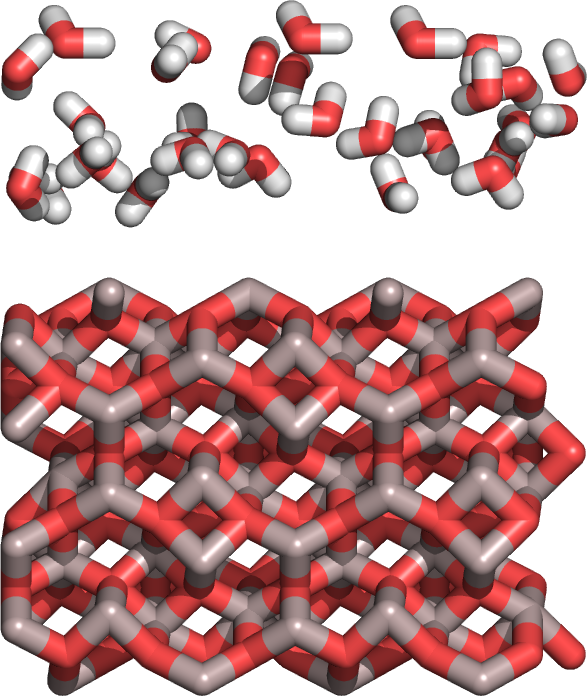
\includegraphics[width=\textwidth]{alumina_h2o_before}
    \subcaption{Seitenansicht, vorher}
  \end{subfigure}
  \hfill
  \begin{subfigure}[t]{\subfigwidth}
    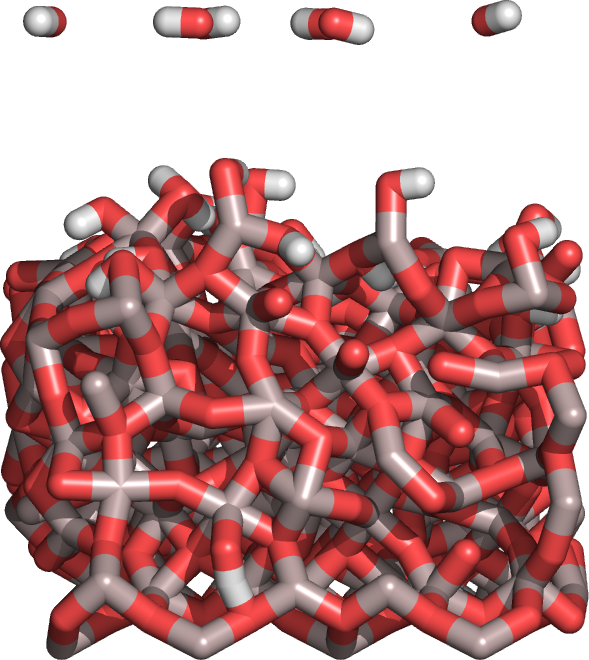
\includegraphics[width=\textwidth]{alumina_h2o_after}
    \subcaption{Seitenansicht, nachher}
  \end{subfigure}
  \hfill
  \begin{subfigure}[t]{\subfigwidth}
    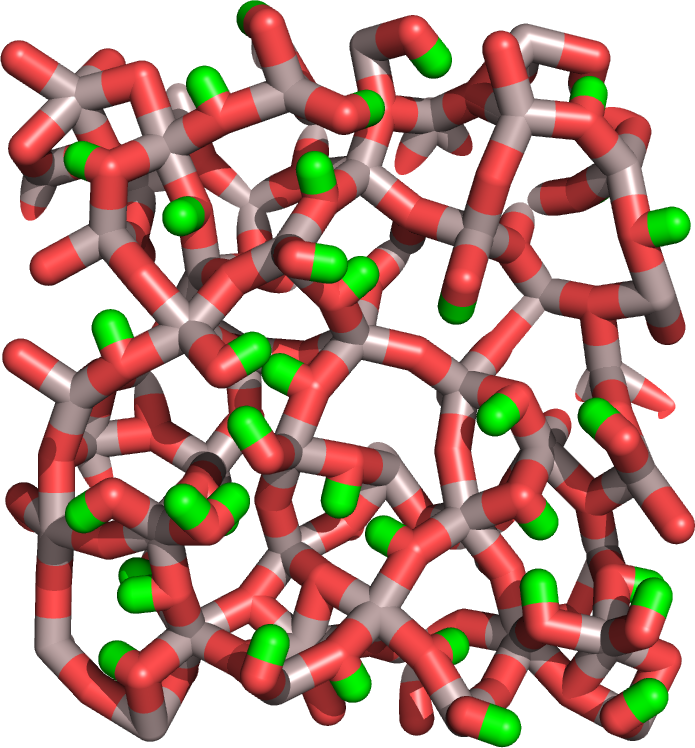
\includegraphics[width=\textwidth]{alumina_h2o_topview}
    \subcaption{Draufsicht, nachher.
      Hydroxyl ist grün hervorgehoben.
    }
  \end{subfigure}
  \caption[Oberflächenreaktion von Wasser mit $\alpha$-\ce{Al2O3}]{Ergebnisse einer Oberflächenreaktion von Wasser mit $\alpha$-\ce{Al2O3}.
    Das Wasser reagiert mit Sauerstoffatomen an der Oberfläche zu Hydroxylgruppen.
  }
  \label{fig:wateraluminasurface}
\end{figure}

\subsection{Vollständige ALD-Simulationen}

\todo[inline]{Erläutern, warum es vermutlich noch nicht geht}
